\section{RTC::Lightweight\-RTObject Interface Reference}
\label{interfaceRTC_1_1LightweightRTObject}\index{RTC::LightweightRTObject@{RTC::LightweightRTObject}}
Lightweight\-RTC::Lightweight\-RTObject interface.  


{\tt import \char`\"{}RTC.idl\char`\"{};}

Inheritance diagram for RTC::Lightweight\-RTObject::\begin{figure}[H]
\begin{center}
\leavevmode
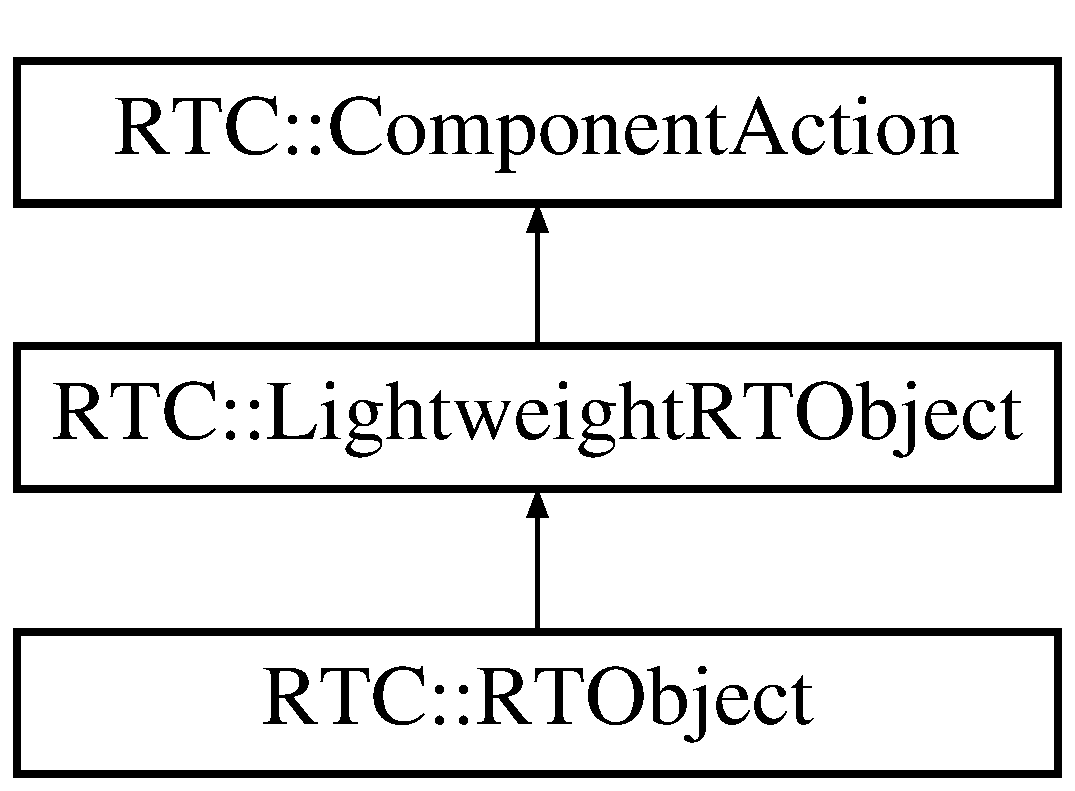
\includegraphics[height=3cm]{interfaceRTC_1_1LightweightRTObject}
\end{center}
\end{figure}
\subsection*{Public Member Functions}
\begin{CompactItemize}
\item 
{\bf Return\-Code\_\-t} {\bf initialize} ()
\item 
{\bf Return\-Code\_\-t} {\bf finalize} ()
\item 
{\bf Return\-Code\_\-t} {\bf exit} ()
\item 
boolean {\bf is\_\-alive} ()
\item 
{\bf Execution\-Context\-List} {\bf get\_\-contexts} ()
\item 
{\bf Execution\-Context} {\bf get\_\-context} (in {\bf Unique\-Id} ec\_\-id)
\item 
{\bf Unique\-Id} {\bf attach\_\-executioncontext} (in {\bf Execution\-Context} exec\_\-context)
\item 
{\bf Return\-Code\_\-t} {\bf detach\_\-executioncontext} (in {\bf Unique\-Id} ec\_\-id)
\item 
{\bf Return\-Code\_\-t} {\bf on\_\-initialize} ()
\item 
{\bf Return\-Code\_\-t} {\bf on\_\-finalize} ()
\item 
{\bf Return\-Code\_\-t} {\bf on\_\-startup} (in {\bf Unique\-Id} ec\_\-id)
\item 
{\bf Return\-Code\_\-t} {\bf on\_\-shutdown} (in {\bf Unique\-Id} ec\_\-id)
\item 
{\bf Return\-Code\_\-t} {\bf on\_\-activated} (in {\bf Unique\-Id} ec\_\-id)
\item 
{\bf Return\-Code\_\-t} {\bf on\_\-deactivated} (in {\bf Unique\-Id} ec\_\-id)
\item 
{\bf Return\-Code\_\-t} {\bf on\_\-aborting} (in {\bf Unique\-Id} ec\_\-id)
\item 
{\bf Return\-Code\_\-t} {\bf on\_\-error} (in {\bf Unique\-Id} ec\_\-id)
\item 
{\bf Return\-Code\_\-t} {\bf on\_\-reset} (in {\bf Unique\-Id} ec\_\-id)
\end{CompactItemize}


\subsection{Detailed Description}
Lightweight\-RTC::Lightweight\-RTObject interface. 



\subsection{Member Function Documentation}
\index{RTC::LightweightRTObject@{RTC::Lightweight\-RTObject}!attach_executioncontext@{attach\_\-executioncontext}}
\index{attach_executioncontext@{attach\_\-executioncontext}!RTC::LightweightRTObject@{RTC::Lightweight\-RTObject}}
\subsubsection{\setlength{\rightskip}{0pt plus 5cm}{\bf Unique\-Id} RTC::Component\-Action::attach\_\-executioncontext (in {\bf Execution\-Context} {\em exec\_\-context})\hspace{0.3cm}{\tt  [inherited]}}\label{interfaceRTC_1_1ComponentAction_RTC_1_1RTObjecta9}


\index{RTC::LightweightRTObject@{RTC::Lightweight\-RTObject}!detach_executioncontext@{detach\_\-executioncontext}}
\index{detach_executioncontext@{detach\_\-executioncontext}!RTC::LightweightRTObject@{RTC::Lightweight\-RTObject}}
\subsubsection{\setlength{\rightskip}{0pt plus 5cm}{\bf Return\-Code\_\-t} RTC::Component\-Action::detach\_\-executioncontext (in {\bf Unique\-Id} {\em ec\_\-id})\hspace{0.3cm}{\tt  [inherited]}}\label{interfaceRTC_1_1ComponentAction_RTC_1_1RTObjecta10}


\index{RTC::LightweightRTObject@{RTC::Lightweight\-RTObject}!exit@{exit}}
\index{exit@{exit}!RTC::LightweightRTObject@{RTC::Lightweight\-RTObject}}
\subsubsection{\setlength{\rightskip}{0pt plus 5cm}{\bf Return\-Code\_\-t} RTC::Lightweight\-RTObject::exit ()}\label{interfaceRTC_1_1LightweightRTObject_RTC_1_1RTObjecta5}


\index{RTC::LightweightRTObject@{RTC::Lightweight\-RTObject}!finalize@{finalize}}
\index{finalize@{finalize}!RTC::LightweightRTObject@{RTC::Lightweight\-RTObject}}
\subsubsection{\setlength{\rightskip}{0pt plus 5cm}{\bf Return\-Code\_\-t} RTC::Lightweight\-RTObject::finalize ()}\label{interfaceRTC_1_1LightweightRTObject_RTC_1_1RTObjecta4}


\index{RTC::LightweightRTObject@{RTC::Lightweight\-RTObject}!get_context@{get\_\-context}}
\index{get_context@{get\_\-context}!RTC::LightweightRTObject@{RTC::Lightweight\-RTObject}}
\subsubsection{\setlength{\rightskip}{0pt plus 5cm}{\bf Execution\-Context} RTC::Lightweight\-RTObject::get\_\-context (in {\bf Unique\-Id} {\em ec\_\-id})}\label{interfaceRTC_1_1LightweightRTObject_RTC_1_1RTObjecta8}


\index{RTC::LightweightRTObject@{RTC::Lightweight\-RTObject}!get_contexts@{get\_\-contexts}}
\index{get_contexts@{get\_\-contexts}!RTC::LightweightRTObject@{RTC::Lightweight\-RTObject}}
\subsubsection{\setlength{\rightskip}{0pt plus 5cm}{\bf Execution\-Context\-List} RTC::Lightweight\-RTObject::get\_\-contexts ()}\label{interfaceRTC_1_1LightweightRTObject_RTC_1_1RTObjecta7}


\index{RTC::LightweightRTObject@{RTC::Lightweight\-RTObject}!initialize@{initialize}}
\index{initialize@{initialize}!RTC::LightweightRTObject@{RTC::Lightweight\-RTObject}}
\subsubsection{\setlength{\rightskip}{0pt plus 5cm}{\bf Return\-Code\_\-t} RTC::Lightweight\-RTObject::initialize ()}\label{interfaceRTC_1_1LightweightRTObject_RTC_1_1RTObjecta3}


\index{RTC::LightweightRTObject@{RTC::Lightweight\-RTObject}!is_alive@{is\_\-alive}}
\index{is_alive@{is\_\-alive}!RTC::LightweightRTObject@{RTC::Lightweight\-RTObject}}
\subsubsection{\setlength{\rightskip}{0pt plus 5cm}boolean RTC::Lightweight\-RTObject::is\_\-alive ()}\label{interfaceRTC_1_1LightweightRTObject_RTC_1_1RTObjecta6}


\index{RTC::LightweightRTObject@{RTC::Lightweight\-RTObject}!on_aborting@{on\_\-aborting}}
\index{on_aborting@{on\_\-aborting}!RTC::LightweightRTObject@{RTC::Lightweight\-RTObject}}
\subsubsection{\setlength{\rightskip}{0pt plus 5cm}{\bf Return\-Code\_\-t} RTC::Component\-Action::on\_\-aborting (in {\bf Unique\-Id} {\em ec\_\-id})\hspace{0.3cm}{\tt  [inherited]}}\label{interfaceRTC_1_1ComponentAction_RTC_1_1RTObjecta17}


\index{RTC::LightweightRTObject@{RTC::Lightweight\-RTObject}!on_activated@{on\_\-activated}}
\index{on_activated@{on\_\-activated}!RTC::LightweightRTObject@{RTC::Lightweight\-RTObject}}
\subsubsection{\setlength{\rightskip}{0pt plus 5cm}{\bf Return\-Code\_\-t} RTC::Component\-Action::on\_\-activated (in {\bf Unique\-Id} {\em ec\_\-id})\hspace{0.3cm}{\tt  [inherited]}}\label{interfaceRTC_1_1ComponentAction_RTC_1_1RTObjecta15}


\index{RTC::LightweightRTObject@{RTC::Lightweight\-RTObject}!on_deactivated@{on\_\-deactivated}}
\index{on_deactivated@{on\_\-deactivated}!RTC::LightweightRTObject@{RTC::Lightweight\-RTObject}}
\subsubsection{\setlength{\rightskip}{0pt plus 5cm}{\bf Return\-Code\_\-t} RTC::Component\-Action::on\_\-deactivated (in {\bf Unique\-Id} {\em ec\_\-id})\hspace{0.3cm}{\tt  [inherited]}}\label{interfaceRTC_1_1ComponentAction_RTC_1_1RTObjecta16}


\index{RTC::LightweightRTObject@{RTC::Lightweight\-RTObject}!on_error@{on\_\-error}}
\index{on_error@{on\_\-error}!RTC::LightweightRTObject@{RTC::Lightweight\-RTObject}}
\subsubsection{\setlength{\rightskip}{0pt plus 5cm}{\bf Return\-Code\_\-t} RTC::Component\-Action::on\_\-error (in {\bf Unique\-Id} {\em ec\_\-id})\hspace{0.3cm}{\tt  [inherited]}}\label{interfaceRTC_1_1ComponentAction_RTC_1_1RTObjecta18}


\index{RTC::LightweightRTObject@{RTC::Lightweight\-RTObject}!on_finalize@{on\_\-finalize}}
\index{on_finalize@{on\_\-finalize}!RTC::LightweightRTObject@{RTC::Lightweight\-RTObject}}
\subsubsection{\setlength{\rightskip}{0pt plus 5cm}{\bf Return\-Code\_\-t} RTC::Component\-Action::on\_\-finalize ()\hspace{0.3cm}{\tt  [inherited]}}\label{interfaceRTC_1_1ComponentAction_RTC_1_1RTObjecta12}


\index{RTC::LightweightRTObject@{RTC::Lightweight\-RTObject}!on_initialize@{on\_\-initialize}}
\index{on_initialize@{on\_\-initialize}!RTC::LightweightRTObject@{RTC::Lightweight\-RTObject}}
\subsubsection{\setlength{\rightskip}{0pt plus 5cm}{\bf Return\-Code\_\-t} RTC::Component\-Action::on\_\-initialize ()\hspace{0.3cm}{\tt  [inherited]}}\label{interfaceRTC_1_1ComponentAction_RTC_1_1RTObjecta11}


\index{RTC::LightweightRTObject@{RTC::Lightweight\-RTObject}!on_reset@{on\_\-reset}}
\index{on_reset@{on\_\-reset}!RTC::LightweightRTObject@{RTC::Lightweight\-RTObject}}
\subsubsection{\setlength{\rightskip}{0pt plus 5cm}{\bf Return\-Code\_\-t} RTC::Component\-Action::on\_\-reset (in {\bf Unique\-Id} {\em ec\_\-id})\hspace{0.3cm}{\tt  [inherited]}}\label{interfaceRTC_1_1ComponentAction_RTC_1_1RTObjecta19}


\index{RTC::LightweightRTObject@{RTC::Lightweight\-RTObject}!on_shutdown@{on\_\-shutdown}}
\index{on_shutdown@{on\_\-shutdown}!RTC::LightweightRTObject@{RTC::Lightweight\-RTObject}}
\subsubsection{\setlength{\rightskip}{0pt plus 5cm}{\bf Return\-Code\_\-t} RTC::Component\-Action::on\_\-shutdown (in {\bf Unique\-Id} {\em ec\_\-id})\hspace{0.3cm}{\tt  [inherited]}}\label{interfaceRTC_1_1ComponentAction_RTC_1_1RTObjecta14}


\index{RTC::LightweightRTObject@{RTC::Lightweight\-RTObject}!on_startup@{on\_\-startup}}
\index{on_startup@{on\_\-startup}!RTC::LightweightRTObject@{RTC::Lightweight\-RTObject}}
\subsubsection{\setlength{\rightskip}{0pt plus 5cm}{\bf Return\-Code\_\-t} RTC::Component\-Action::on\_\-startup (in {\bf Unique\-Id} {\em ec\_\-id})\hspace{0.3cm}{\tt  [inherited]}}\label{interfaceRTC_1_1ComponentAction_RTC_1_1RTObjecta13}




The documentation for this interface was generated from the following file:\begin{CompactItemize}
\item 
{\bf RTC.idl}\end{CompactItemize}
